\chapter{Wazuh UI}
\section{Startseite}
Auf der Startseite sieht man alle aktiven und inaktiven Computer, die mit dem Wazuh Manager verbunden sind.
Von hier aus hat man Schnellzugriff auf alle ``Module'', die Wazuh anbietet.

\section{Security events}
Im Module Security Events werden alle Alerts angezeigt, welche durch die definierten Regeln ausgelöst werden.

\begin{figure}[H]
    \centering
    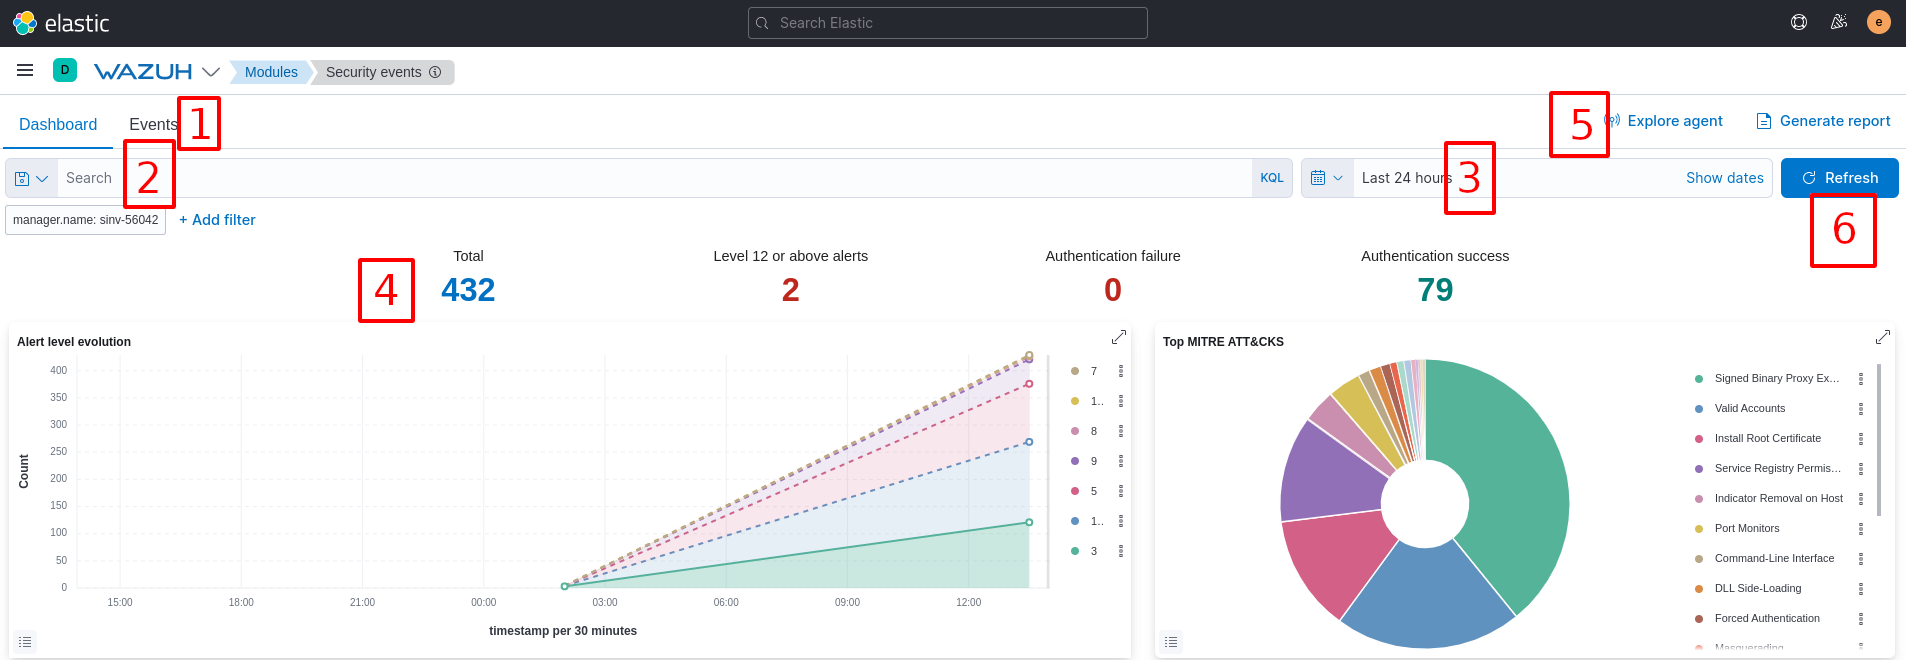
\includegraphics[width=\linewidth]{../img/wazuh-se-1.png}
    \caption{Security Events}
\end{figure}

\begin{enumerate}
    \item Hier kann man zwischen dem Dashboard und den Events wechseln. Das Dashboard zeigt die Alerts und zusammenfassende Diagramme an. Unter Events sieht man nur die Alerts, dafür aber zusätzlich bessere Filter.
    \item In diesem Eingabefeld kann man die Alerts durchsuchen. Mithilfe von Filtern kann man zum Beispiel gewisse Alerts ausblenden oder nur gewisse Anzeigen lassen.
    \item Hier kann man die Zeitspanne angeben, wie lange Zurück man die Alerts ansehen möchte.
    \item Diese Übersicht zeigt an, 
\end{enumerate}

\section{Integrity Monitoring}
